\documentclass[]{article}
\usepackage[margin=1.15in]{geometry}
\usepackage{setspace}
\usepackage{graphicx}
\usepackage{hyperref}
\usepackage{array}
\usepackage{float}
\usepackage{caption}
\usepackage{multirow}

\onehalfspacing
%opening
\title{ParkMe: Hazard Analysis}
\author{Daniel Agostinho\\agostd - 001414323\\ Group 5 \and Michael Bitzos\\bitzosm - 001405050\\ Group 5 \and Kathryn Brownlee\\brownlks - 001408416\\ Group 5  \and Anthony Chang\\changa7 - 001413615\\ Group 5 \and Ben Petkovsek\\petkovb - 001417104\\ Group 5}


\begin{document}
\date{March 4, 2019}
\maketitle
\begin{center}
\begin{table}[b]
\centering
\begin{tabular}{|c|c|}
 \hline
 Revision & Date \\ 
 \hline
 Rev0 & November 4, 2018 \\ 
 Rev1 & February 28, 2019 \\ 
 \hline
\end{tabular}
\end{table}
\end{center}
\newpage
\tableofcontents
\newpage
\listoffigures
\listoftables
\newpage

\captionsetup{font=bf}

\section{Introduction}
Although ParkMe has very little physical interaction with the environment and the users, like most products, there is still inherent risk that comes with the system. The assumption is that the user will be driving for most of the interaction of the system. The system needs to ensure that it does not pose a risk to the driver, nor cause the driver to be distracted and further cause damage with their vehicle.


\subsection{Scope}
The victims of these hazards are not limited to just the driver and others in cars. Damage may also occur to pedestrians, other stationary vehicles, the physical sensors for the system, and infrastructure of the parking lot. All of these potential victims must be accounted for in analyzing the hazards of the system. Although the system cannot directly harm the user, there are control actions that the system makes that can have consequences that will lead to an accident or a loss. The correctness of the system’s sensing and output of the sensor data/ geographical location is imperative for the safe use of the system. Thus the control actions that are within the scope of the hazard analysis are the ones that are directly responsible for receiving and outputting the information to the user.


\subsection{Purpose}
This document serves to outline the hazards associated with the product ParkMe. The hazard analysis technique that will be used for this document is the STPA technique. First we will identify the main control actions that can be hazardous. Then for each control action we will determine the hazards that come with those actions. We will breakdown the system control actions by component as can be seen in Figure 1. Finally the consequences of the hazards will be shown in the consequence matrix in Table 2.

\begin{figure}[H]
	\centering
	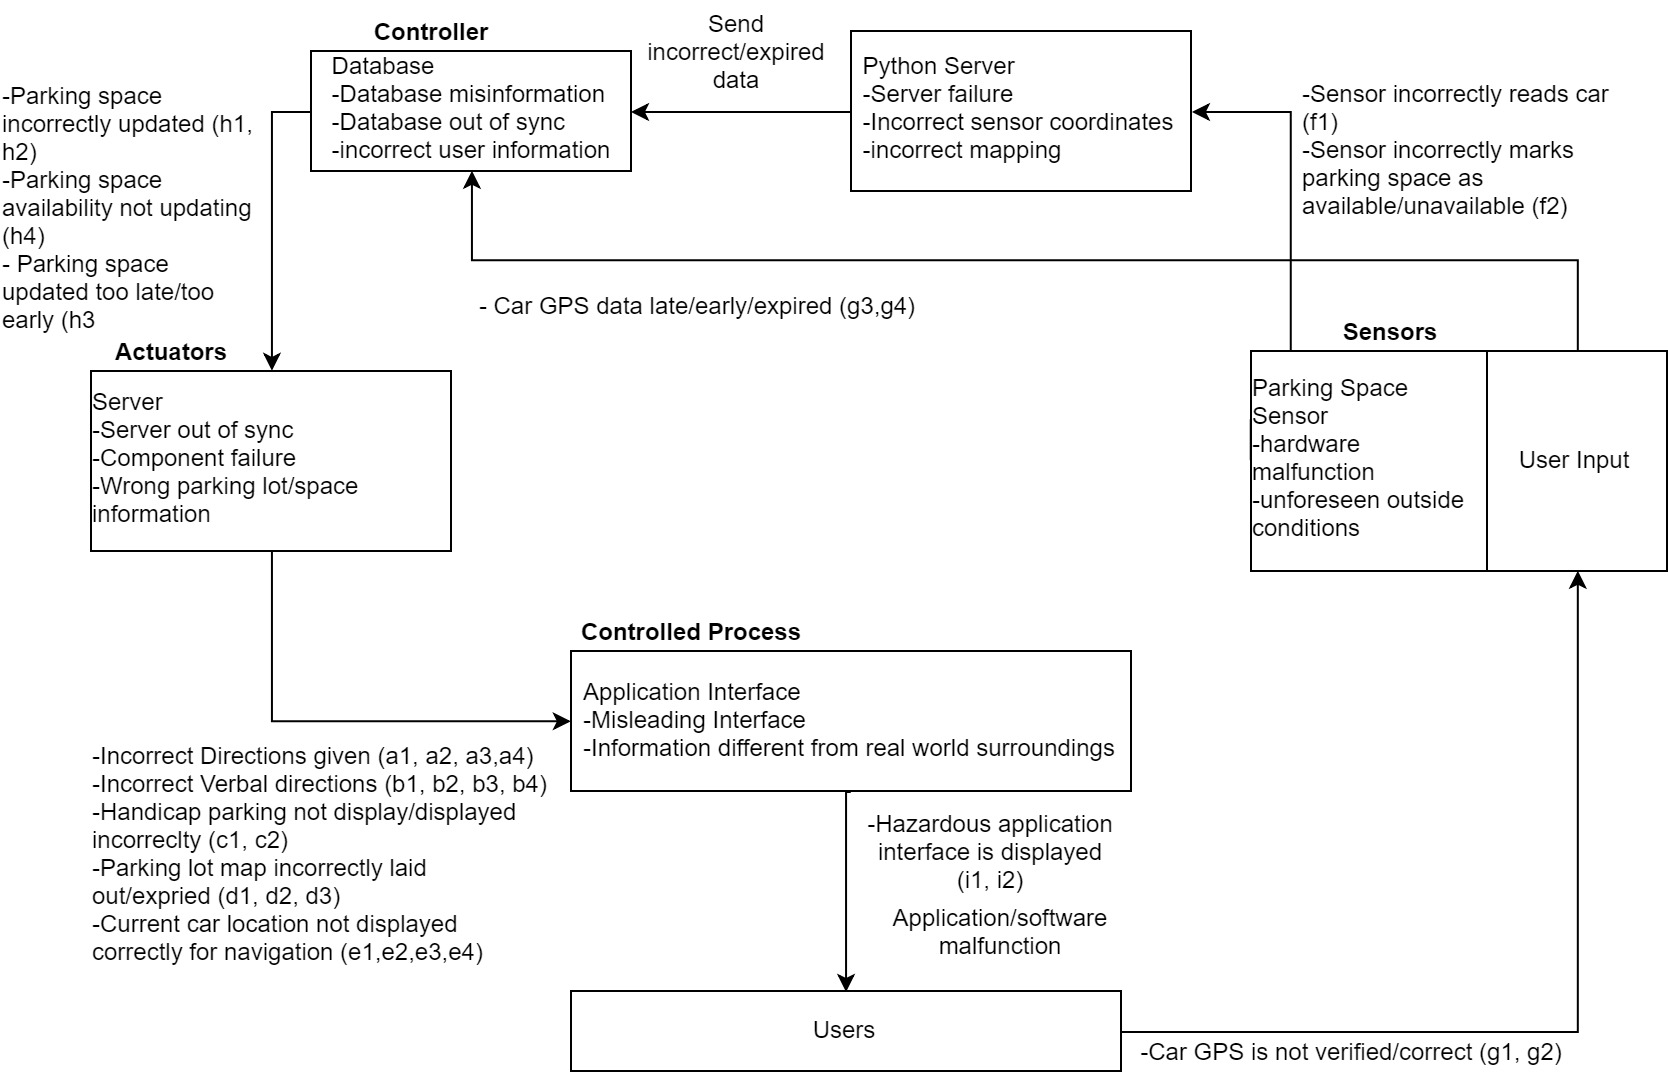
\includegraphics[width=\textwidth,height=\textheight,keepaspectratio]{images/stpa}
	\caption{STPA breakdown of system control actions and hazards.}
	\label{fig:fdd}
\end{figure}


\begin{table}
	\begin{tabular}{ | m{2.5cm} | m{3cm}| m{3cm}| m{3cm}| m{3cm} |} 
		\hline
		Control Action & 
		Category 1: A control action required for safety is not provided or is not followed.
		 & 
		 Category 2: an unsafe control action is provided that leads to a hazard
		  & 
		  Category 3: A potentially safe control action is provided too early, too late, or out of sequence
		   & 
		   Category 4: A safe control action is stopped too soon.
		    \\ [0.5ex] 
		\hline
		Display Map Directions (A) & Necessary direction is missing. (a1) & Provided direction of navigation is wrong. (a2) & Turns or stops are provided at the wrong time. (a3) & Directions are stopped while driving. (a4) \\ 
		\hline
		Provide voice navigation (B) & Verbal direction does not match physical location. (b1) & Verbal direction does not match physical location. (b2)
	 & Verbal direction timing does not match physical location. (b3) & Verbal directions are stopped while driving. (b4) \\ 
		\hline 
		Display Handicap Parking (C) & Handicap Parking spot not displayed to user. (c1) & Handicap parking spot is displayed incorrectly. (c2) & N/A & N/A \\
		\hline
		Display Available Parking Spots (D) & Map of parking lot is missing/ incorrect. (d1) & Map of parking lot is incorrect or misleading. (d2) & Map of parking lot is displayed while user is not within range of parking lot. Map of parking lot does not display on time when user is within range. (d3) & N/A \\	
		\hline
		Update Car Location on Map (E) & Car is not displayed on screen. (e1) & Car location is not displayed to match current physical location within acceptable bounds. (e2) & Car location is not updated within acceptable timing range. (e3) & Car location display ends before user arrival. (e4) \\	
		\hline
		Sense Car in Spot (F) & System fails to read data from sensor. (f1) & The sensors incorrectly sense the parking spot. (f2) & N/A & N/A \\	
		\hline
		Get Car Location (G) & Car GPS coordinates are unavailable. (g1) & GPS coordinates do not match current physical location within acceptable bounds. (g2) & GPS coordinates are not updated within acceptable frequency. (g3) & GPS Coordinates stop being provided before arrival. (g4) \\	
		\hline
		Update Spot Availability (H) & The availability of a spot is not updated when it changes. (h1) & A spot is said to be available when it isn’t or vice-versa. (h2) & Spot is not updated within acceptable time range. (h3) & Spot availability is not updated. (h4) \\	
		\hline
		Application interface display (I) & Application display is not functional (I1) & Application displays incorrect information. (i2) & N/A & N/A \\	
		\hline
	\end{tabular}
	\caption{Monitored Variables for ParkMe.}
\end{table}

	\begin{table}
		\begin{tabular}{ | m{2.5cm} | m{3cm}| m{3cm}| m{3cm}| m{3cm} |} 
			\hline
			Control Action & 
			Consequence of Hazard I
			& 
			Consequence of Hazard II
			& 
			Consequence of Hazard III
			& 
			Consequence of Hazard IV
			\\ [0.5ex] 
			\hline
			Display Map Directions (A) & Could result in dangerous maneuvers or incorrect turns. May result in distracted driving, leading to crash, damage of property, personal harm or harms of others. & Could result in dangerous maneuvers or incorrect turns. May result in distracted driving, leading to crash, damage of property, personal harm or harms of others.
			& Could result in dangerous maneuvers or incorrect turns. May result in distracted driving, leading to crash, damage of property, personal harm or harms of others. & Could result in dangerous maneuvers or incorrect turns. May result in distracted driving, leading to crash, damage of property, personal harm or harms of others. \\ 
			\hline 
			Provide voice navigation (B) & Could result in dangerous maneuvers or incorrect turns. May result in distracted driving, leading to crash, damage of property, personal harm or harms of others. & Could result in dangerous maneuvers or incorrect turns. May result in distracted driving, leading to crash, damage of property, personal harm or harms of others.
			& Could result in dangerous maneuvers or incorrect turns. May result in distracted driving, leading to crash, damage of property, personal harm or harms of others. & Could result in dangerous maneuvers or incorrect turns. May result in distracted driving, leading to crash, damage of property, personal harm or harms of others. \\ 
			\hline 
			Display Handicap Parking (C) & User may erroneously park in a handicap spot. & Handicap user may be led to non-handicap spot. & N/A & N/A \\
			\hline
			Display Available Parking Spots (D) &May result in distracted driving, leading to crash, damage of property, personal harm or harms of others. & May result in distracted driving, leading to crash, damage of property, personal harm or harms of others. & May result in distracted driving, leading to crash, damage of property, personal harm or harms of others. & N/A \\		
			\hline
		\end{tabular}
		\caption{Consequence Matrix Part I.}
 \end{table}
\begin{table}
	\begin{tabular}{ | m{2.5cm} | m{3cm}| m{3cm}| m{3cm}| m{3cm} |} 
		\hline
		Control Action & 
		Consequence of Hazard I
		& 
		Consequence of Hazard II
		& 
		Consequence of Hazard III
		& 
		Consequence of Hazard IV
		\\ [0.5ex]
		\hline
		Update Car Location on Map (E) & May result in distracted driving, leading to crash, damage of property, personal harm or harms of others. & Could result in dangerous maneuvers or incorrect turns. Driver may drive into vehicle, private property or physical obstruction if they are not vigilant.  & Could result in dangerous maneuvers or incorrect turns. Driver may drive into vehicle, private property or physical obstruction if they are not vigilant.  & Could result in dangerous maneuvers or incorrect turns. Driver may drive into vehicle, private property or physical obstruction if they are not vigilant.  \\	
		\hline
		Sense Car in Spot (F) & Driver may drive into vehicle, private property or physical obstruction if they are not vigilant. & Driver may drive into vehicle, private property or physical obstruction if they are not vigilant. (f2) & N/A & N/A \\ 
		\hline
		Get Car Location (G) & Could result in dangerous maneuvers or incorrect turns. May result in distracted driving, leading to crash, damage of property, personal harm or harms of others. & Could result in dangerous maneuvers or incorrect turns. May result in distracted driving, leading to crash, damage of property, personal harm or harms of others. & Could result in dangerous maneuvers or incorrect turns. May result in distracted driving, leading to crash, damage of property, personal harm or harms of others. & Could result in dangerous maneuvers or incorrect turns. May result in distracted driving, leading to crash, damage of property, personal harm or harms of others.  \\	
		\hline
		Update Spot Availability (H) & Driver may drive into vehicle, private property or physical obstruction if they are not vigilant.& Driver may drive into vehicle, private property or physical obstruction if they are not vigilant. & Driver may drive into vehicle, private property or physical obstruction if they are not vigilant. & Driver may drive into vehicle, private property or physical obstruction if they are not vigilant.  \\	
		\hline
		Application interface display (I) & May result in distracted driving, leading to crash, damage of property, personal harm or harms of others. & May result in distracted driving, leading to crash, damage of property, personal harm or harms of others. & N/A & N/A \\	
		\hline
	\end{tabular}
\caption{Consequence Matrix Part II.}
\end{table}
\begin{table}
	\begin{tabular}{ | m{2.5cm} | m{12cm} |} 
		\hline
		Hazard ID & 
		Hazard Mitigation Strategy
		\\ [0.5ex]
		\hline 
		a1 & Calculate map route multiple times to ensure direction is displayed or if there is a valid error. \\	
		\hline 
		a2 & Calculate map route multiple times to ensure direction is displayed or if there is a valid error. \\	
		\hline 
		a3 & Ensure directions are provided within a certain threshold of time, and if not recalculate directions instantly. \\	
		\hline 
		a4 & Recalculate navigation when directions have halted. \\	
		\hline 
		b1 & Allow user to submit feedback for correction. \\	
		\hline 
		b2 & Allow user to submit feedback for correction. \\	
		\hline 
		b3 & Allow user to submit feedback for correction. \\	
		\hline 
		b4 & Restart voice navigation if it has halted before destination has been reached or not cancelled. \\	
		\hline 
		c1 & Warn user to be aware of surroundings. \\	
		\hline 
		c2 & Warn user to be aware of surroundings. \\	
		\hline 
		d1 & Implement runtime checking for missing maps and redundant checking for incorrect layouts. \\	
		\hline 
		d2 & Implement runtime checking for missing maps and redundant checking for incorrect layouts. \\	
		\hline 
		d3 & Check in real time for GPS distance to parking lot and display map accordingly.  \\
		\hline 
		e1 & Warn user on application startup to be aware of their surroundings.  \\
		\hline 
		e2 & Constantly check GPS coordinates and update the application display accordingly.  \\
		\hline 
		e3 & Constantly check GPS coordinates and update the application display accordingly.  \\
		\hline 
		e4 & Constantly check GPS coordinates and update the application display accordingly. \\
		\hline 
		f1 & Send multiple update packets from sensor for redundancy  \\
		\hline 
		f2 & Implement multiple sensors per parking spot for redundant parking detection.  \\	
		\hline 
		g1 & Attempt to acquire GPS location data multiple times. Notify user if GPS location data is unavailable. \\	
		\hline 
		g2 & Allow user to manually refresh GPS location data to acquire new coordinates.  \\	
		\hline 
		g3 & Increase update frequency (based on testing and user feedback)  \\	
		\hline 
		g4 & Attempt to acquire GPS location data multiple times. Notify user if GPS location data is unavailable.  \\	
		\hline 
		h1 & Increase update frequency with server and display time last updated. \\	
		\hline 
		h2 & Increase update frequency with server and display time last updated.  \\	
		\hline 
		h3 & Increase update frequency (based on testing and user feedback)  \\	
		\hline 
		h4 & Attempt to update spot availability multiple times when failed and display time last updated \\	
		\hline 
		i1 & Attempt to display application when error detected. Close application if application is unable to be displayed.   \\	
		\hline 
		i2 & Periodically update from server for latest information. Allow user to submit feedback for correction.  \\	
		
		
		\hline
	\end{tabular}
	\caption{Hazard Mitigation Table.}
\end{table}



\end{document}
